% Compile with XeLaTeX:
%   xelatex main.tex
% or:
%   latexmk -xelatex main.tex
%
% Figures used by this report are copied into ./figures for self-contained compilation.

\documentclass[UTF8,a4paper,12pt]{ctexart}

\usepackage[a4paper,margin=2.3cm]{geometry}
\usepackage{amsmath}
\usepackage{array}
\usepackage{booktabs}
\usepackage{float}
\usepackage{graphicx}
\usepackage{hyperref}
\usepackage{longtable}
\usepackage{multirow}
\usepackage{subcaption}

\hypersetup{
  colorlinks=true,
  linkcolor=black,
  citecolor=black,
  urlcolor=blue
}

\title{基于脑启发核心集选择的轻量级 VLA 机械臂动作预测}
\author{
  姓名：\underline{\hspace{4cm}} \\
  学号：\underline{\hspace{4cm}} \\
  专业班级：\underline{\hspace{4cm}}
}
\date{2026年6月}

\begin{document}

\maketitle

\begin{abstract}
本文围绕《视觉认知工程》课程题目二“基于脑启发核心集选择的轻量级 VLA 机械臂动作预测”展开研究。题目指出，视觉-语言-动作模型在真实遥操作训练中普遍面临“数据冗余与算力墙”问题：连续多帧画面变化很小、简单动作片段占比过高、操作者犹豫和噪声会引入次优样本，若直接在全量数据上训练，不仅计算代价较高，也可能削弱模型泛化能力。受人脑预测编码机制和效用过滤机制启发，本文尝试通过数据修剪与核心集选择，在低算力条件下保留对动作学习最有价值的样本。

本文使用 \texttt{lerobot/aloha\_sim\_transfer\_cube\_human} 数据集。该数据集包含 50 条成功的人类演示轨迹，总体规模较小、结构标准化，适合课程作业中的轻量级验证。实验中选取顶视角图像 \texttt{observation.images.top} 作为视觉输入，并将 14 维双臂动作裁剪为左臂 7 自由度动作标签，构建动作回归任务。本文采用冻结的 ResNet-18 提取图像特征，并使用统一的 MLP 回归器比较随机 10\% 采样、动作变化采样、视觉变化采样、视觉与动作联合采样、脑启发核心集采样以及全量训练的效果。实验结果表明，在相同 10\% 数据比例下，脑启发核心集方法取得了 $0.002603$ 的测试集动作 MSE，优于随机 10\% 的 $0.002829$，相对下降约 $8.0\%$；而全量训练的测试 MSE 为 $0.002368$。该结果说明，将“预测误差敏感性”和“分布多样性”结合起来进行样本筛选，能够在小样本训练场景中更有效地保留关键视觉-动作样本，并为低成本 VLA 数据筛选提供一种具有认知启发意义的可行思路。
\end{abstract}

\tableofcontents

\section{研究背景与问题定义}

视觉-语言-动作模型（Vision-Language-Action, VLA）是具身智能中的关键模型形式，其目标是将环境图像、任务语义和机器人状态映射到底层动作控制信号。在机械臂操作任务中，VLA 模型通常需要处理连续图像帧、语言任务描述以及机械臂关节或末端执行器状态，并预测下一步动作或一段动作序列。因此，VLA 实际上承担着“从多模态感知到端到端动作决策”的核心角色。

然而，真实机器人操作数据并不总是高效的监督信号。根据背景机制调研，在人类遥操作采集的数据中，至少存在以下三类典型问题。

第一类是\textbf{时序冗余}。机械臂执行任务时，相邻帧之间的视觉变化通常较小，尤其是在等待、缓慢接近目标、动作完成后的稳定阶段，大量连续帧携带的信息高度重复。如果将这些帧全部用于训练，模型会反复学习近似相同的样本，计算开销上升，但对动作预测性能的增益有限。

第二类是\textbf{分布冗余}。在操作数据中，不同阶段的样本分布往往并不均衡。例如，在抓取类任务中，“接近目标”“保持匀速移动”这类简单状态可能占据大量比例，而真正影响任务成败的关键状态，如接触物体、夹爪闭合、抓取后转移、目标放置等，出现次数反而较少。如果训练数据过度集中于简单状态，模型就可能对关键操作阶段学习不足。

第三类是\textbf{次优噪声}。人类遥操作数据中常包含犹豫、回退、微调、抖动甚至局部不稳定动作。这些数据虽然来自成功轨迹，但并不意味着每一帧都对学习稳定控制策略有正向作用。对于参数规模较小的轻量级模型而言，过多低效样本和噪声样本可能会干扰动作回归，使模型学习到不稳定的映射关系。

因此，在低算力场景下，与其简单依赖更大规模的数据，不如优先筛选\textbf{高价值样本}。所谓核心集选择，本质上是在较小的数据子集上尽量保留原始数据中的关键分布、关键状态变化和关键动作阶段，以减少训练成本，同时尽可能维持甚至提升模型效果。

从视觉认知工程视角来看，这一问题可以借助两类脑启发机制来理解。

\subsection{预测编码：为什么要关注“变化大的时刻”}

预测编码（Predictive Coding）认为，大脑并不是被动接受所有输入，而是持续根据当前状态对下一时刻感知进行预测。当真实输入与预测结果高度一致时，神经系统只需要较弱响应；而当真实输入显著偏离预测时，预测误差信号会增强，从而引导更多认知资源聚焦到变化显著的位置或时刻。

将这一思想映射到机器人操作数据中，可以得到一种直观的时序过滤原则：如果相邻帧之间的视觉特征和动作标签变化很小，则这些帧的信息增量有限，可以视为低价值样本；如果某一帧相对于前后帧出现明显变化，则说明它更可能对应状态转换或关键操作时刻，因而具有更高保留价值。也正因为如此，本文后续将视觉变化和动作变化作为样本评分的核心成分。

\subsection{网状激活系统：为什么不能只看“变化大”}

仅仅关注变化量仍然不够。网状激活系统（Reticular Activating System, RAS）与生物认知中的觉醒、注意调节和信息筛选有关。面对复杂环境时，人类不会平均处理所有感官输入，而是会根据当前任务目标，将认知资源分配给更重要的信息。例如，在抓取任务中，人类更关注目标物体、机械臂末端、接触点及动作转折区域，而不是与任务无关的背景细节。

对应到 VLA 数据筛选中，这意味着样本的重要性不仅取决于“是否发生变化”，还取决于“这种变化是否与任务目标相关”。某些视觉变化可能只是背景扰动，并不一定有助于动作预测；反之，某些接触、抓取、夹爪切换、放置等关键阶段，即便只持续较短时间，也应当被优先保留。因此，本文后续在高效用候选池之外，还加入了分布覆盖与多样性选择，避免只保留少量高度相似的高变化样本。

\subsection{研究问题}

基于上述分析，本文关注的不是“如何训练一个更大的 VLA 模型”，而是“如何在轻量级设置下更高效地利用数据”。具体而言，本文希望回答以下问题：
\begin{enumerate}
  \item 在 ALOHA 仿真操作数据中，视觉变化和动作变化能否作为样本信息价值的有效指标？
  \item 在相同 10\% 数据预算下，脑启发核心集选择是否优于随机采样？
  \item 如果同时考虑高效用筛选和分布多样性，是否能够更好地保留对动作预测真正有帮助的关键样本？
\end{enumerate}

因此，本文尝试将预测编码启发的“变化敏感性”和 RAS 启发的“任务效用过滤”结合起来：先利用视觉变化与动作变化估计样本效用，再在高效用候选池中加入多样性约束，构造 10\% 的脑启发核心集，并与随机 10\% 采样进行比较。

\section{任务与数据集}

\subsection{数据集说明}

实验使用的数据集为 \texttt{lerobot/aloha\_sim\_transfer\_cube\_human}。该数据集包含 50 条成功的人类演示轨迹，每条轨迹包含多视角相机图像、机器人状态信息和 14 维双臂动作标签。考虑到课程作业更强调实验闭环与结果分析，而非训练完整大型 VLA 模型，本文选择顶视角图像作为视觉输入，并将动作标签裁剪为左臂前 7 维，构成单臂动作回归任务。

\subsection{任务构建}

最终训练样本可表示为：
\[
x = [\text{image\_feature}, \text{language\_feature}], \qquad
y = [a_1, a_2, a_3, a_4, a_5, a_6, a_7].
\]

其中，\texttt{image\_feature} 为冻结视觉模型提取的图像特征，\texttt{language\_feature} 采用常量任务编码。由于本数据集本质上接近单任务演示，因此本文不引入复杂语言编码器，而是将重点放在视觉-动作数据核心集筛选本身。

\section{方法设计}

\subsection{冻结视觉特征提取}

本文使用 ImageNet 预训练的 ResNet-18 作为视觉特征提取器，移除最终分类层后输出 512 维图像特征，并保持其参数冻结。这样做有两个原因：第一，ResNet-18 体量较小，适合课程作业中的低算力场景；第二，冻结特征提取器可以将实验重点集中在“数据选择是否有效”这一问题上。

本文最终输入特征维度为 513，其中 512 维来自图像特征，1 维来自常量语言编码。

\subsection{数据划分与训练模型}

为了避免同一条轨迹中的帧同时出现在训练集和测试集中，本文采用 episode-level 划分，将全部轨迹按 80\%/10\%/10\% 划分为 train、val、test。核心集选择仅在训练集内部进行，验证集和测试集在所有方法之间保持一致。

动作预测模型统一采用轻量级 MLP 回归器，其结构为：
\[
513 \rightarrow 512 \rightarrow 256 \rightarrow 7.
\]

训练配置如下：
\begin{itemize}
  \item 优化器：AdamW
  \item 学习率：$1\times10^{-3}$
  \item 权重衰减：$1\times10^{-4}$
  \item batch size：256
  \item 最大训练轮数：100
  \item early stopping patience：15
  \item 损失函数：MSELoss
\end{itemize}

所有方法共享完全相同的模型结构和训练超参数，确保实验变量只来自数据选择策略。

\subsection{脑启发核心集选择策略}

本文设计的核心思想是：高价值样本应同时满足“包含明显状态变化”和“具有一定分布代表性”。

首先，定义视觉变化分数：
\[
\text{visual\_change}_t = \lVert f_t - f_{t-1} \rVert_2,
\]
其中 $f_t$ 表示第 $t$ 帧的视觉特征。视觉变化越大，说明当前帧与前一帧差异越明显，通常对应更强的预测误差信号。

其次，定义动作变化分数：
\[
\text{action\_change}_t = \lVert a_t - a_{t-1} \rVert_2,
\]
其中 $a_t$ 表示第 $t$ 帧的动作向量。动作变化越大，说明该时刻更可能处于任务执行中的关键控制阶段。

在训练集范围内对两个分数进行标准化后，构造样本效用：
\[
\text{utility}_t
= \lambda_v \cdot z(\text{visual\_change}_t)
 +\,
  \lambda_a \cdot z(\text{action\_change}_t).
\]

实验中取 $\lambda_v = 1.0$、$\lambda_a = 1.0$。在此基础上，本文采用两阶段核心集选择：
\begin{enumerate}
  \item 在训练集中按 \texttt{utility} 从高到低排序，取前 30\% 样本作为候选池。
  \item 在候选池内执行 KMeans 聚类，以目标样本数作为聚类数，从每个簇中选择距离中心较近且效用较高的样本。
\end{enumerate}

该设计的作用是同时兼顾“高信息量”和“分布覆盖度”，避免只挑出少量高度相似的突变帧。与之对应，本文还实现了 \texttt{random}、\texttt{action\_change}、\texttt{visual\_change} 和 \texttt{visual\_action} 作为对比方法。

\section{实验设置}

\subsection{对比方法}

本文比较以下 6 种方法：
\begin{enumerate}
  \item \texttt{random}：在训练集中按 episode 配额随机抽取 10\% 样本；
  \item \texttt{action\_change}：优先选择动作变化最大的 10\% 样本；
  \item \texttt{visual\_change}：优先选择视觉变化最大的 10\% 样本；
  \item \texttt{visual\_action}：基于视觉变化与动作变化联合分数进行选择；
  \item \texttt{brain\_coreset}：高效用候选池 + KMeans 多样性选择；
  \item \texttt{full}：使用 100\% 训练数据。
\end{enumerate}

\subsection{评价指标}

本文采用动作预测的均方误差（MSE）作为主指标，并同时观察验证集与测试集表现。由于课程作业重点在于比较不同数据选择策略，因此本文以测试集原始动作空间 MSE 作为主要结论依据。

\section{实验结果}

\subsection{总体结果}

表~\ref{tab:main-results} 给出了所有方法在验证集和测试集上的结果。

\begin{table}[H]
  \centering
  \caption{不同数据选择方法的动作预测结果}
  \label{tab:main-results}
  \begin{tabular}{lccc}
    \toprule
    方法 & 训练样本数 & Val MSE & Test MSE \\
    \midrule
    Action Change 10\% & 1600 & 0.007216 & 0.004999 \\
    Visual Change 10\% & 1600 & 0.006072 & 0.003051 \\
    Visual + Action 10\% & 1600 & 0.005850 & 0.003892 \\
    Random 10\% & 1600 & 0.003749 & 0.002829 \\
    Brain-inspired Coreset 10\% & 1600 & 0.004267 & 0.002603 \\
    Full 100\% & 16000 & 0.003608 & 0.002368 \\
    \bottomrule
  \end{tabular}
\end{table}

从测试集结果看，各方法从优到劣排序如下：
\[
\texttt{full} < \texttt{brain\_coreset} < \texttt{random} < \texttt{visual\_change} < \texttt{visual\_action} < \texttt{action\_change}.
\]

其中，\texttt{brain\_coreset} 在 10\% 数据量条件下取得 $0.002603$ 的测试 MSE，相比 \texttt{random} 的 $0.002829$，绝对下降 $0.000226$，相对下降约 $8.0\%$。虽然 \texttt{full} 方法仍然取得最优结果 $0.002368$，但与 \texttt{brain\_coreset} 的差距仅约为 $9.0\%$。考虑到 \texttt{brain\_coreset} 只使用了十分之一的数据，这一结果说明在小样本场景中，数据质量可以在一定程度上弥补数据规模不足。

\subsection{结果分析}

首先，单独基于动作变化的 \texttt{action\_change} 表现最差。这说明仅依据动作幅值变化来定义“重要样本”是不够的，因为大动作变化并不一定对应可泛化的视觉-动作映射，也可能过度偏向少数突变片段，忽略了稳定控制阶段中的必要上下文。

其次，\texttt{visual\_change} 明显优于 \texttt{action\_change}，说明视觉预测误差信号比纯动作变化更接近样本的信息价值。这与预测编码理论是一致的：状态变化大的帧通常包含新的环境信息，更值得保留。

第三，简单地将视觉变化和动作变化线性相加形成 \texttt{visual\_action}，结果反而不如随机 10\%。这说明“高效用”本身并不等于“好核心集”。如果缺少多样性约束，模型可能只看到大量相似的高变化帧，造成覆盖面不足。

第四，\texttt{brain\_coreset} 之所以优于 \texttt{random}，关键不只是打分，而是“候选池 + 聚类覆盖”这一两阶段机制。它既保留了具有显著状态变化的关键时刻，又避免了候选样本过度集中在少量局部区域。

\subsection{每维动作误差分析}

从每维测试 MSE 来看，\texttt{brain\_coreset} 在多数维度上优于 \texttt{random}。例如：
\begin{itemize}
  \item 第二维：$0.001210 < 0.001293$
  \item 第三维：$0.000626 < 0.000697$
  \item 第四维：$0.000846 < 0.000890$
  \item 第五维：$0.001873 < 0.002011$
  \item 第七维：$0.011914 < 0.013193$
\end{itemize}

仅第六维略高于随机方法，但整体平均测试误差仍然更低。该现象说明脑启发核心集选择带来的收益并非集中在单一维度，而是多数动作维度上的整体改进。

\section{可视化结果}

\begin{figure}[H]
  \centering
  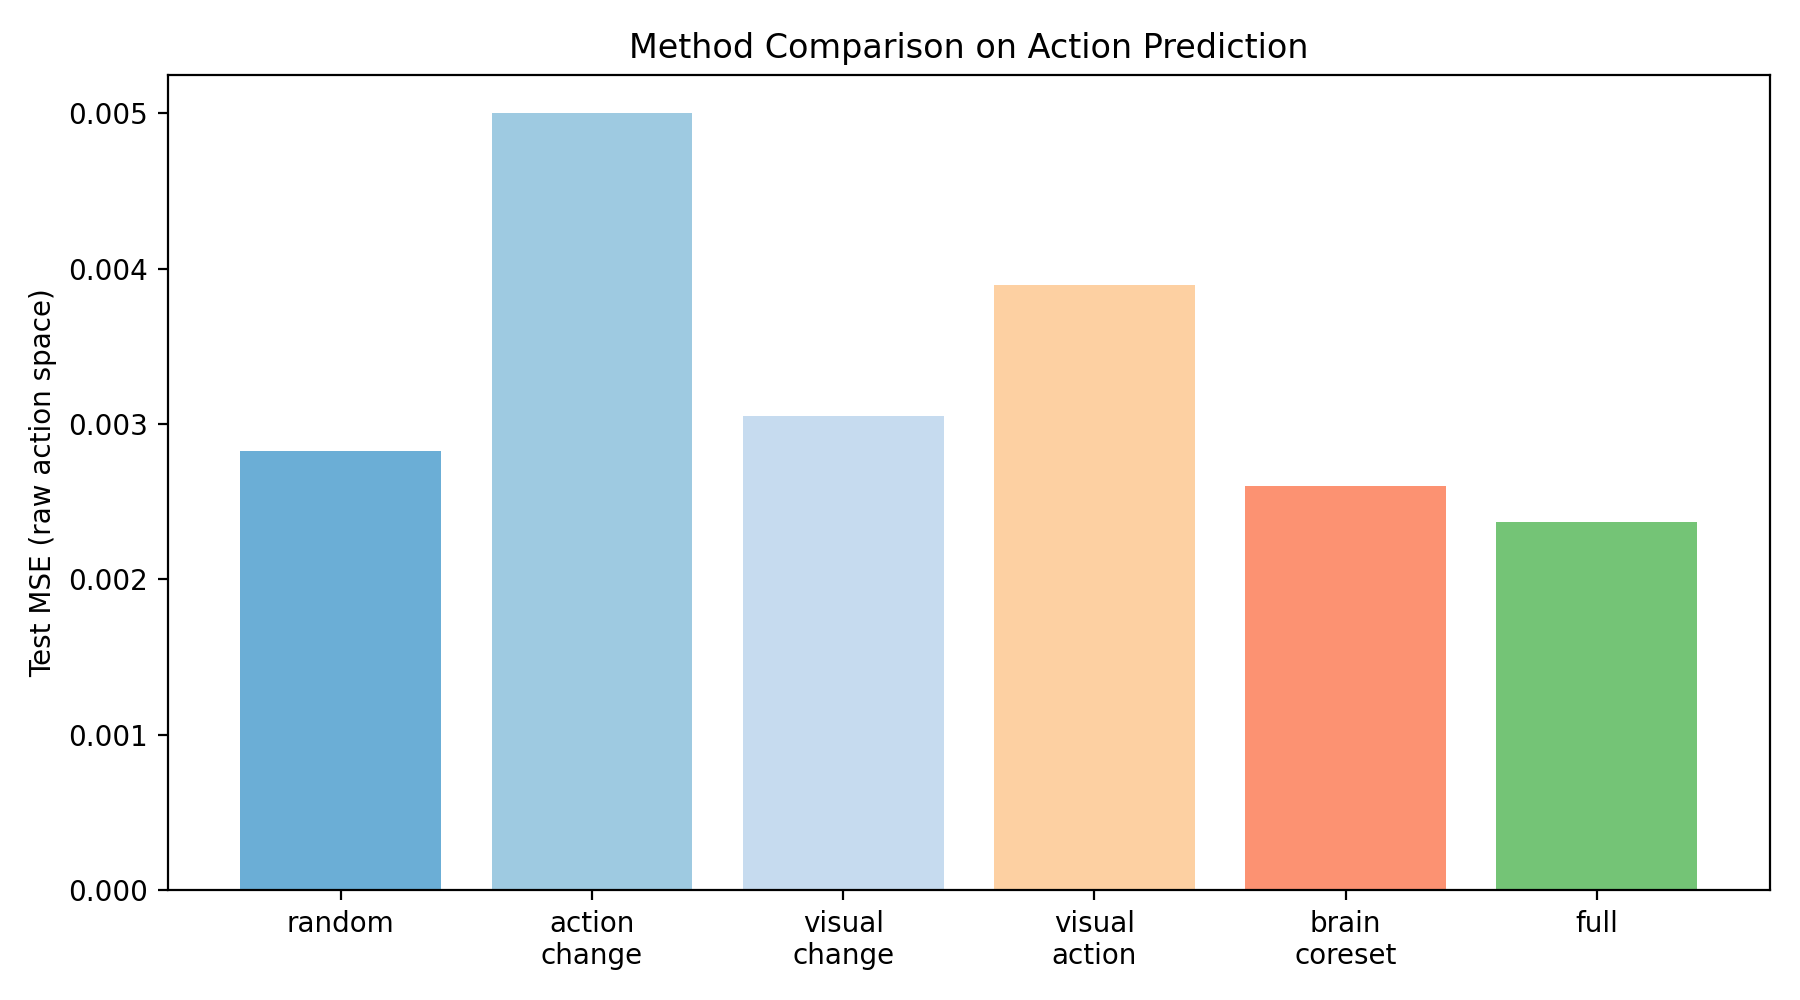
\includegraphics[width=0.72\linewidth]{figures/mse_bar.png}
  \caption{不同数据选择方法的测试集动作 MSE 对比}
  \label{fig:mse-bar}
\end{figure}

\begin{figure}[H]
  \centering
  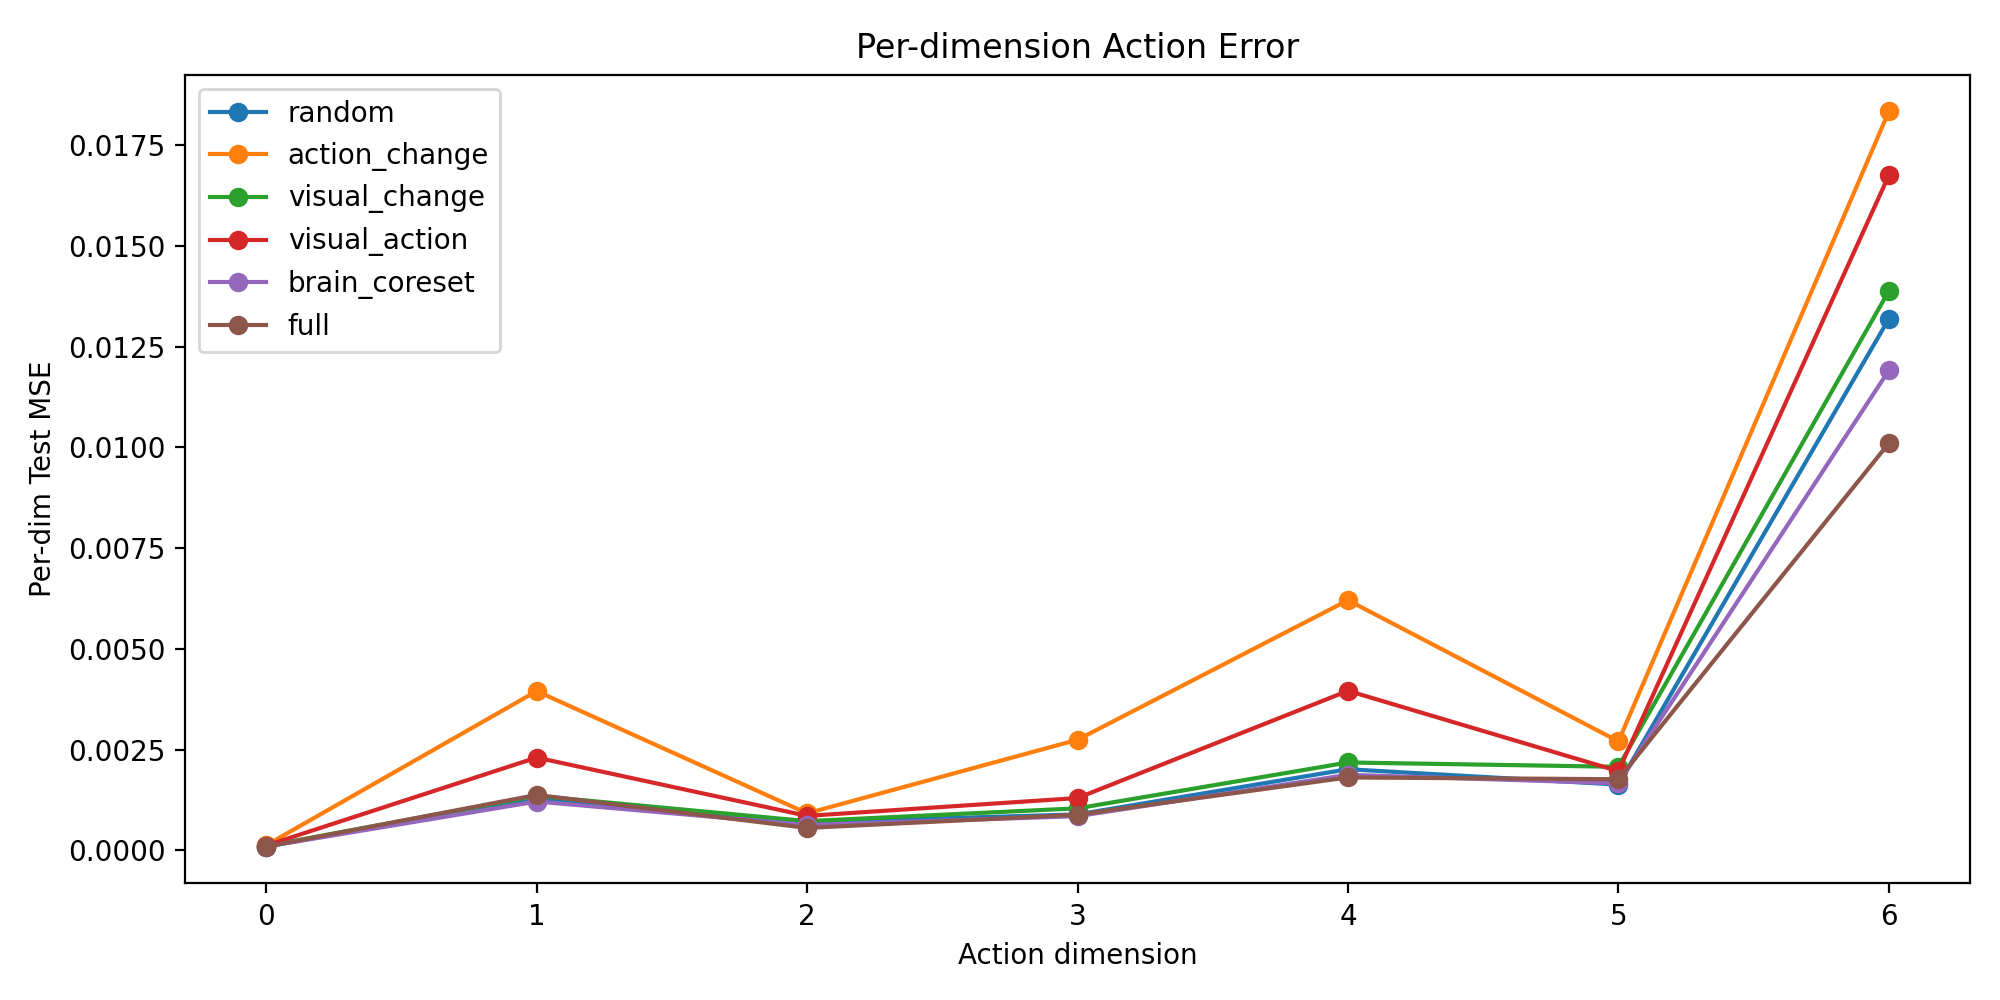
\includegraphics[width=0.78\linewidth]{figures/per_dim_mse.png}
  \caption{不同方法在各动作维度上的测试误差}
  \label{fig:per-dim}
\end{figure}

\begin{figure}[H]
  \centering
  \begin{subfigure}{0.48\linewidth}
    \centering
    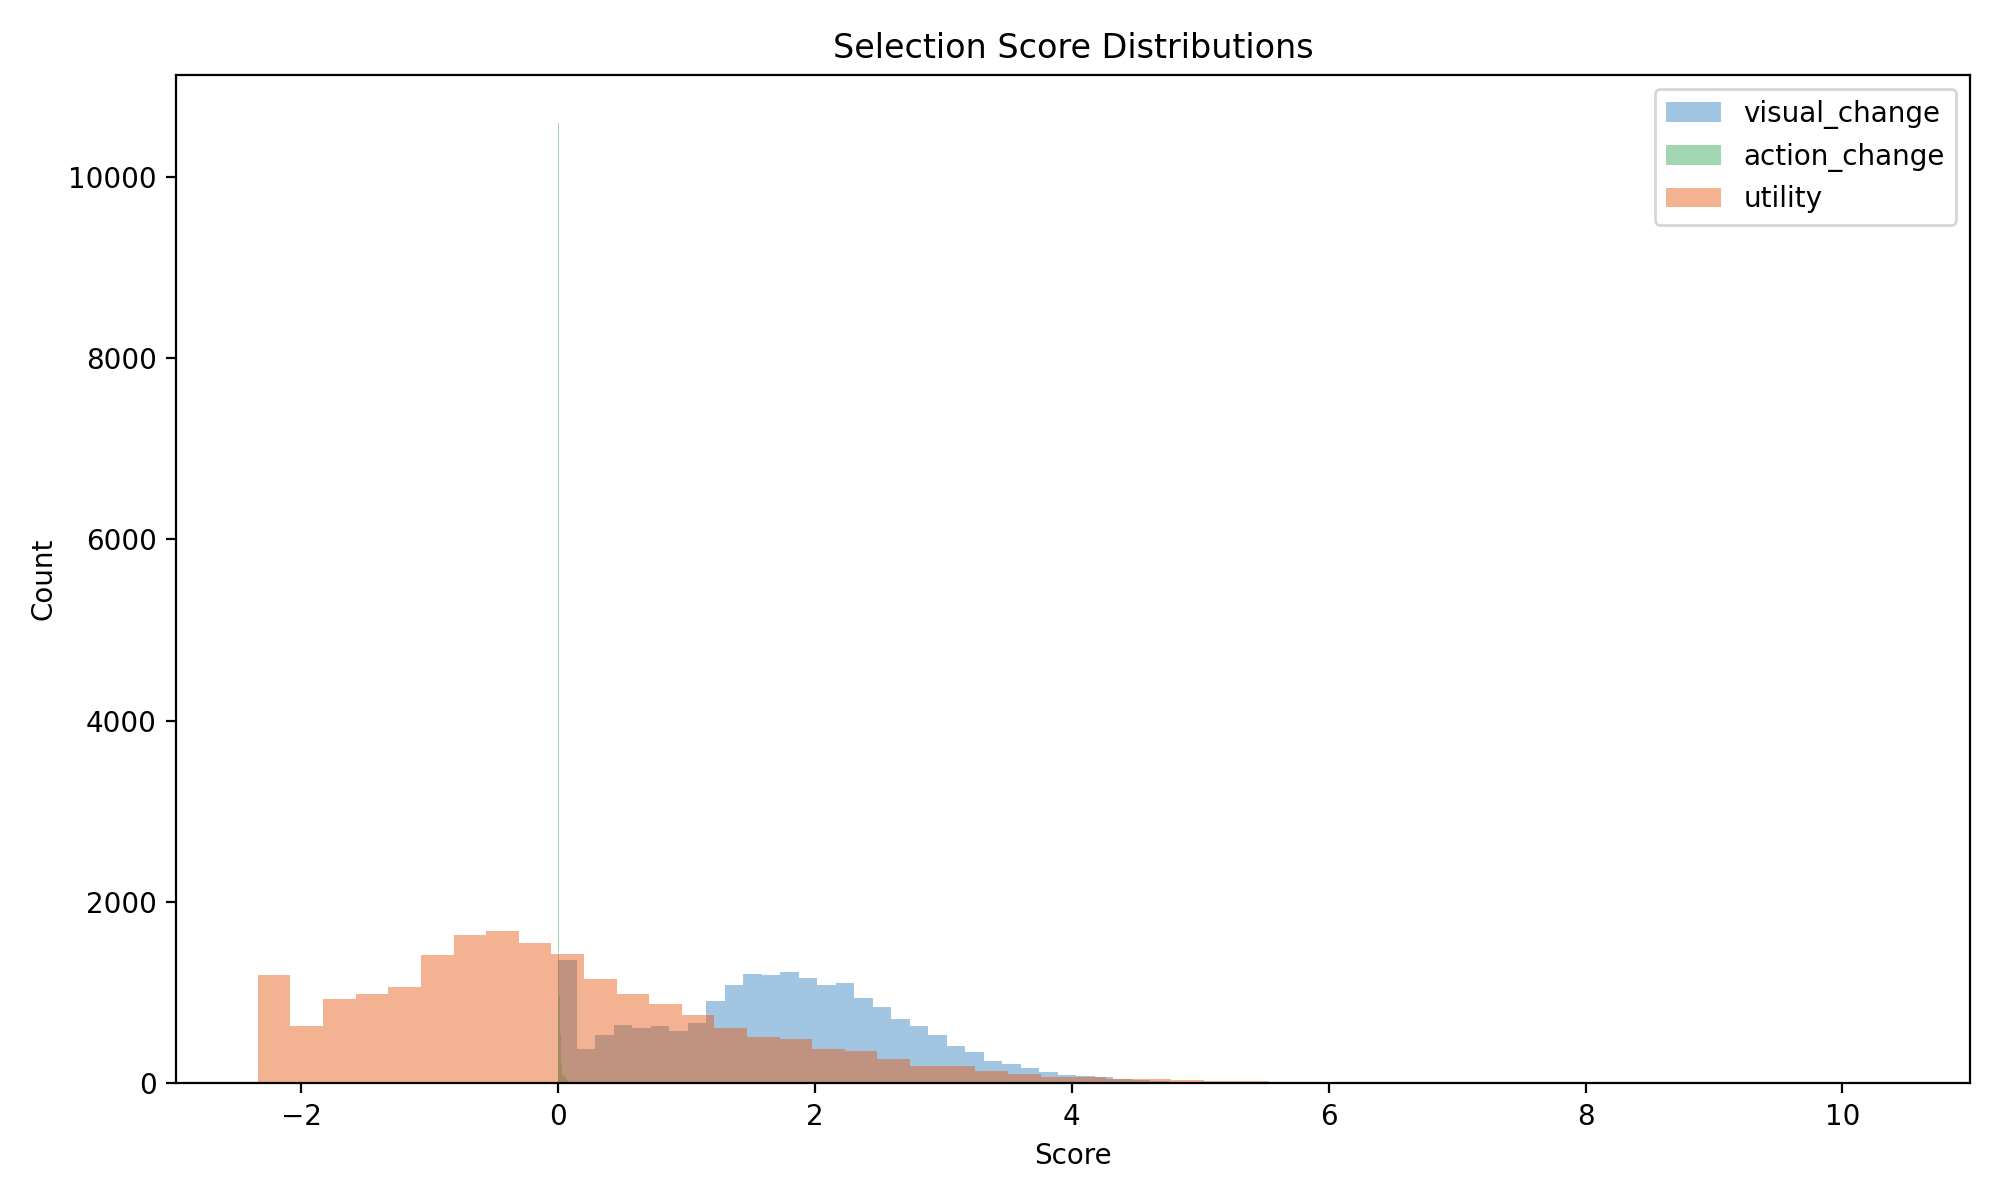
\includegraphics[width=\linewidth]{figures/score_distribution.png}
    \caption{选择分数分布}
  \end{subfigure}
  \begin{subfigure}{0.48\linewidth}
    \centering
    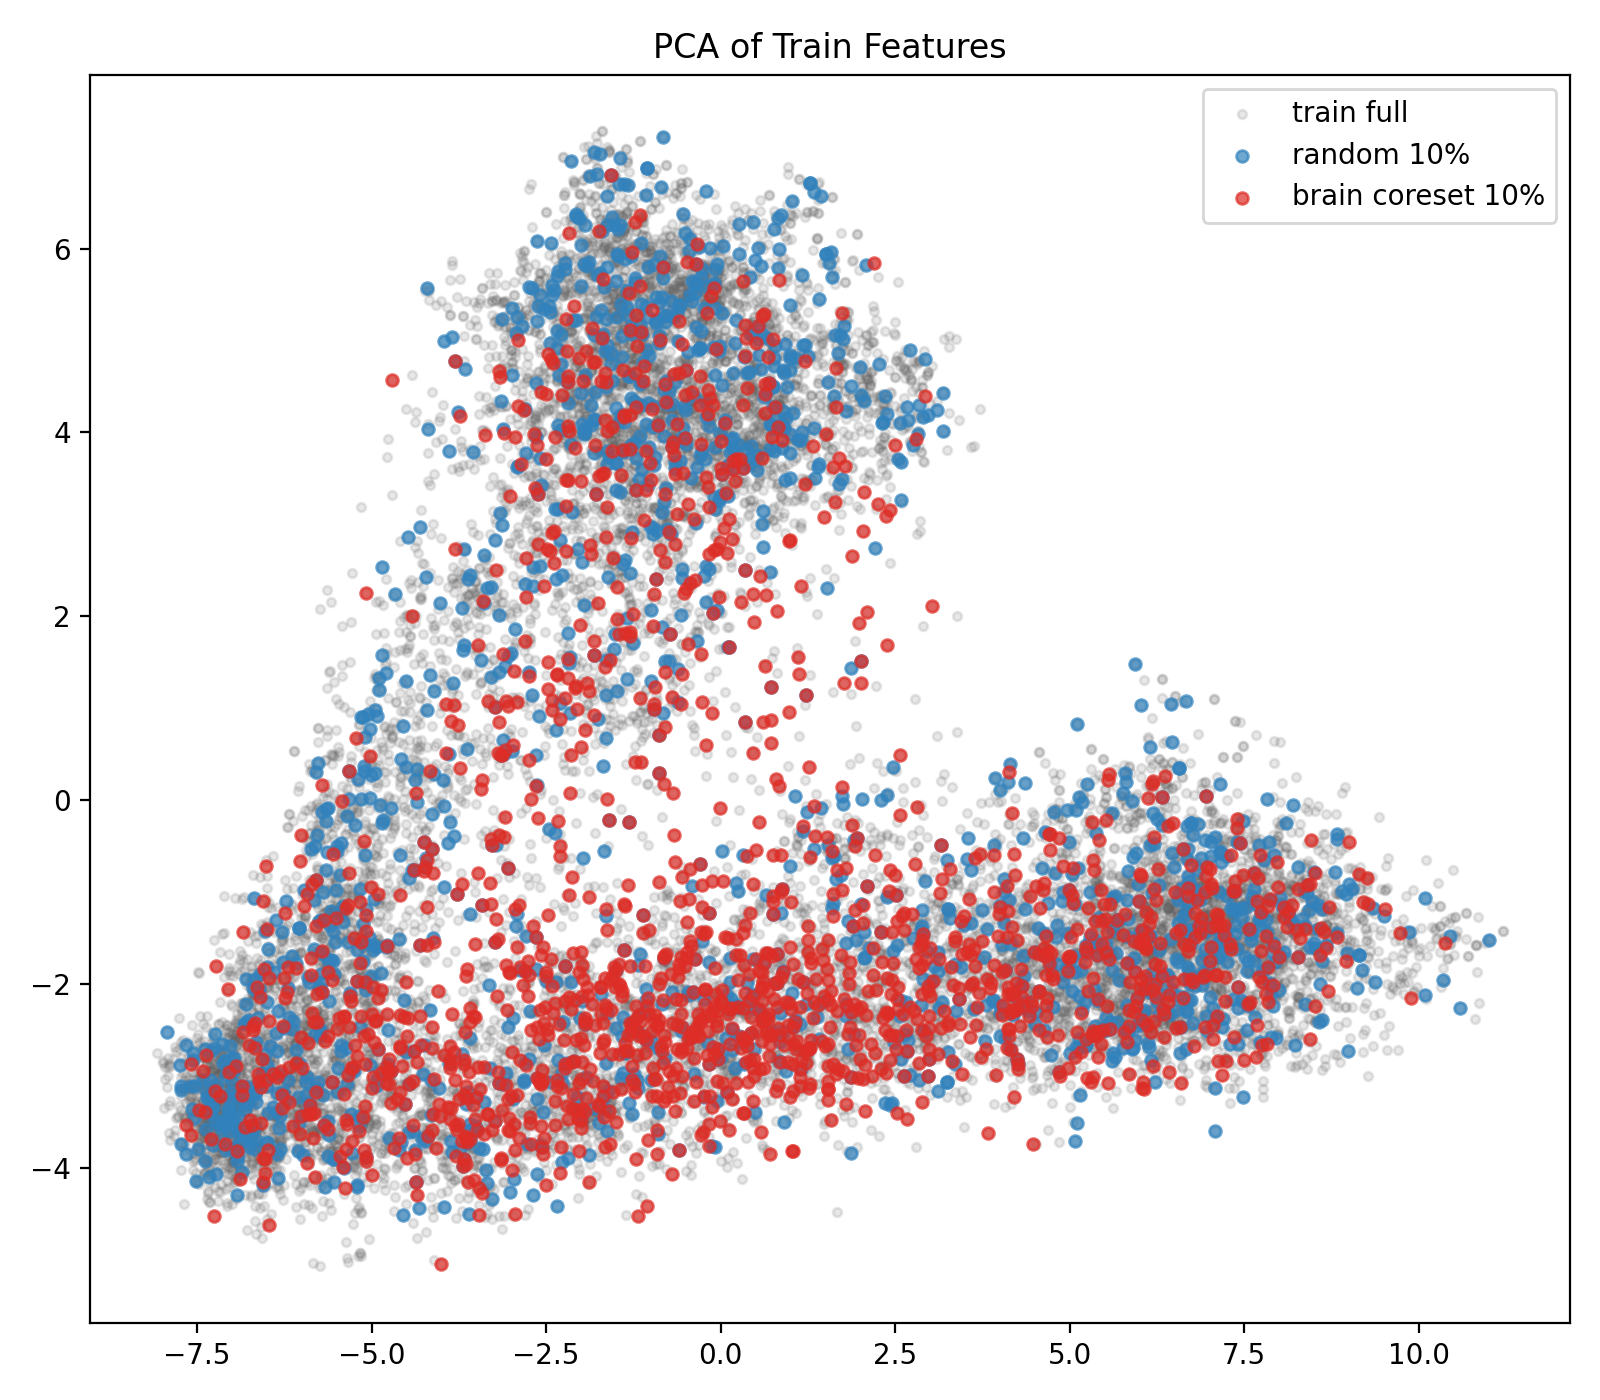
\includegraphics[width=\linewidth]{figures/feature_pca.png}
    \caption{训练特征 PCA 分布}
  \end{subfigure}
  \caption{核心集分数与特征覆盖情况}
  \label{fig:score-pca}
\end{figure}

\begin{figure}[H]
  \centering
  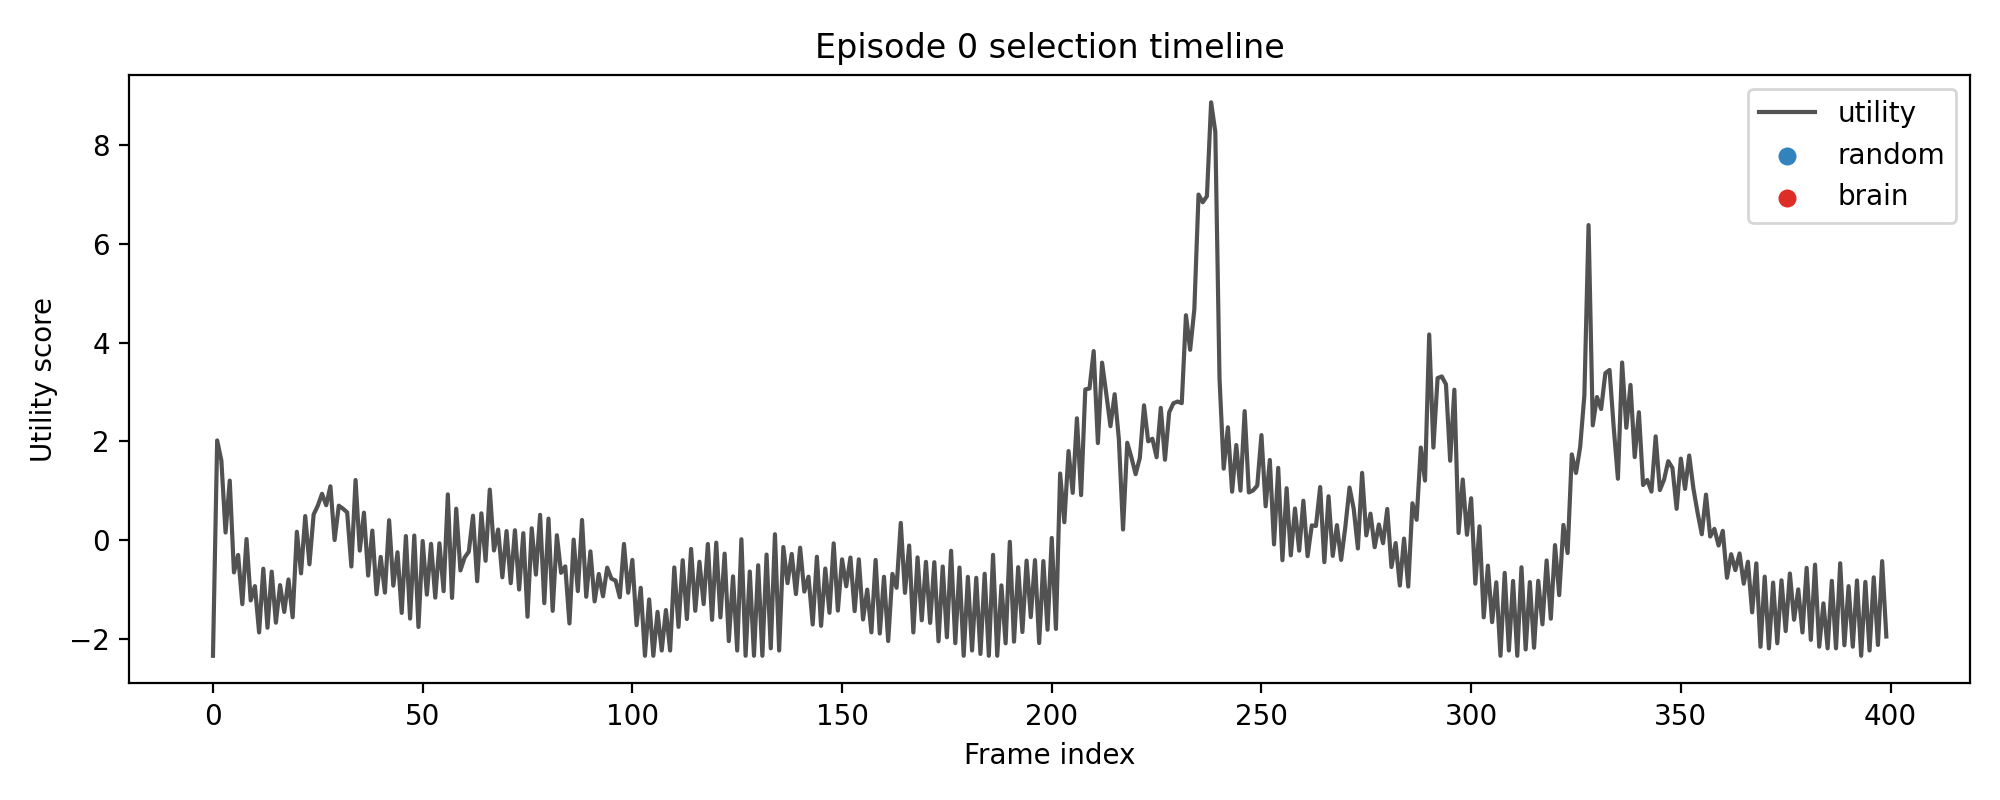
\includegraphics[width=0.78\linewidth]{figures/selection_timeline_episode_0.png}
  \caption{示例 episode 中的 utility 变化与样本选择位置}
  \label{fig:timeline}
\end{figure}

从这些图可以直观支持本文结论：随机采样虽然保留了一定分布覆盖，但不能稳定保留关键变化时刻；单纯高分采样虽然强调“突变帧”，却容易损失多样性；脑启发核心集则在两者之间取得了较好的平衡。

\section{视觉认知机制解释}

\subsection{预测编码}

预测编码认为，大脑更重视与当前预测不一致的输入。对应到本实验中，视觉变化大的帧意味着场景状态发生了值得关注的改变，例如方块位置变化、机械臂接近接触物体、抓取姿态切换等。这些帧对于动作预测模型更有训练价值。

\subsection{效用过滤与注意选择}

在动作执行过程中，动作变化大的时刻往往对应任务中的关键控制阶段，例如接近目标、闭合夹爪、移动和放置。将动作变化纳入 utility 评分，可以视作对“任务相关时刻”的筛选。

\subsection{分布覆盖}

仅关注高变化帧会导致样本集中。加入 KMeans 多样性选择后，核心集不再只保留少数高度相似的关键帧，而是覆盖训练分布中的多个区域。这更接近真实认知系统中“既关注突发信息，也维持场景整体表征”的策略。

\section{局限性与改进方向}

尽管本文结果已经验证了脑启发核心集选择在 10\% 数据量下优于随机采样，但仍存在以下局限：
\begin{enumerate}
  \item 只使用了单随机种子，结果还缺少统计稳定性验证；
  \item 语言特征采用常量编码，没有考察多指令条件下的 VLA 泛化问题；
  \item 视觉特征仅使用 ResNet-18，后续可以比较 CLIP 等更强的冻结编码器；
  \item 核心集方法仍然是启发式设计，尚未引入更严格的优化目标或在线选择机制；
  \item 评估指标仅为动作 MSE，未来可以增加轨迹重建误差或下游任务成功率指标。
\end{enumerate}

未来可以从三个方向继续改进：一是增加多随机种子实验，提升结果可信度；二是将当前静态 coreset 扩展为训练过程中的动态样本选择；三是进一步结合语言信息或机器人状态信息，构建更加完整的多模态核心集方法。

\section{结论}

本文基于 \texttt{lerobot/aloha\_sim\_transfer\_cube\_human} 数据集，完成了一个轻量级、可复现的 VLA 动作预测实验闭环。通过冻结 ResNet-18 提取视觉特征，并在统一 MLP 回归器上比较不同采样策略，本文验证了以下结论：
\begin{enumerate}
  \item 在相同 10\% 数据比例下，脑启发核心集方法优于随机采样；
  \item 仅依据动作变化或简单联合分数进行选择，并不能稳定提升性能；
  \item 将“高效用筛选”和“分布多样性”结合起来，是提升小样本训练效果的关键。
\end{enumerate}

因此，本文支持这样一个课程层面的结论：对于轻量级 VLA 动作预测任务，数据质量并不只是“去掉一些样本”这么简单，而是需要从认知启发角度重新定义什么样的样本更值得保留。脑启发核心集选择正是朝这个方向迈出的一步。

\begin{thebibliography}{99}

\bibitem{act}
Zhao T Z, Kumar V, Levine S, et al.
Learning Fine-Grained Bimanual Manipulation with Low-Cost Hardware (ACT).
Robotics: Science and Systems, 2023.

\bibitem{pruning}
Sorscher B, Geirhos R, Shekhar S, et al.
Beyond neural scaling laws: beating power law scaling via data pruning.
Advances in Neural Information Processing Systems, 2022.

\bibitem{openvla}
Kim M J, Pertsch K, Karamcheti S, et al.
OpenVLA: An Open-Source Vision-Language-Action Model.
arXiv preprint arXiv:2406.09246, 2024.

\bibitem{predictivecoding}
Millidge B, Seth A, Buckley C L.
Predictive coding: a theoretical and experimental review.
arXiv preprint arXiv:2107.12979, 2021.

\end{thebibliography}

\end{document}
